%!TEX root = ../../main.tex
\section{Magnetresonanztomographie (MRT)}
Die \ac{MRT}, auch Kernspintomographie genannt, ist ein bildgebendes Verfahren zur Darstellung von Struktur und Funktion der Weichteile und Organe des Körpers. Mit einer \ac{MRT} können Schnittbilder des Körpers oder einzelner Körperteile erstellt werden. Für die Bildgebung werden starke Magnetfelder verwendet, die jedoch für den menschlichen Körper unschädlich sind, da bei diesem Verfahren keine \gls{Ionisierende Strahlung} verwendet wird. \cite[vgl.][]{Kramme2016}\\
\begin{figure}[ht]
	\centering
	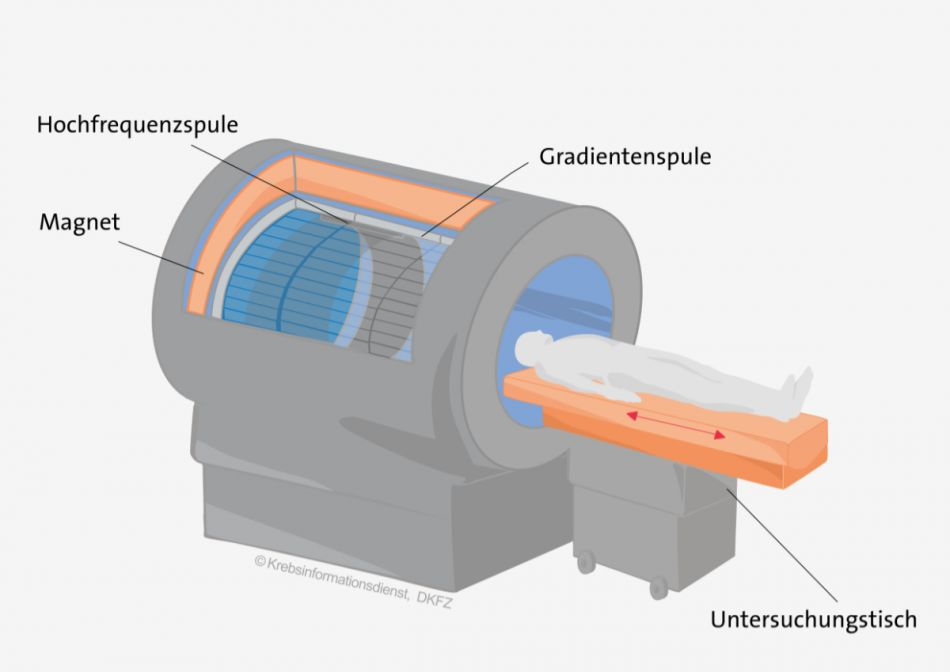
\includegraphics[width=.9\textwidth]{mrt_aufbau.jpg}
	\caption{Schematischer Aufbau eines Magnetresonanztomographen (Quelle: \url{https://www.krebsinformationsdienst.de/untersuchung/bildgebung/kernspintomographie.php})}
\end{figure}

Der Magnetresonanztomograph besteht aus mehreren Komponenten: 
\begin{itemize}
	\item einem supraleitenden Hauptmagneten in einer Röhre, der ein starkes und konstanten Magnetfeld erzeugt. Ein supraleitender Magnet wird durch flüssigen Stickstoff gekühlt, sodass der Spulenwiderstand nahezu null wird. Dies ermöglicht die Erzeugung starker Magnetfelder.
	\item einem Gradientensystem, das zusätzliche Magnetfelder generiert, die je nach Position im Körper unterschiedlich sind und so eine räumliche Auflösung ermöglichen.
	\item einem Hochfrequenzsystem, welches aus einem Sende- und Empfangsspulensystem besteht. Dieses sendet Radiowellen zur Anregung der Wasserstoffatome aus, welche dadurch ihrer Ausrichtung verlieren.
	\item einem Computersystem, das geeignet ist für die Verarbeitung der Daten eines \ac{MRT}s
	\item und einem Untersuchungstisch, auf welchem der Patient während der Untersuchung liegt
\end{itemize}
Das Verfahren beruht auf dem physikalischen Prinzip des Eigendrehimpulses, auch Spin genannt. Ein \gls{Proton} dreht sich um seinen eigenen Schwerpunkt (Kernspin) und erzeugt dabei ein Magnetfeld. Auch die Wasserstoffkerne in unserem Körper besitzen einen Spin und verhalten sich wie kleine Magnete, die ein messbares Magnetfeld erzeugen.\\
Im Normalzustand sind die Kernspins ungeordnet, legt man jedoch ein starkes Magnetfeld an, richten sich die Kernspinachsen entlang der Magnetfeldlinien aus. Dabei führen sie eine Kreiselbewegung aus, bei der sie sich den Feldlinien immer weiter annähern, sich aber nie ganz mit ihnen ausrichten. Die Frequenz dieser Bewegung wird Larmorfrequenz genannt.\\ 
Die Ausrichtung der Kernspins allein reicht nicht aus, um ein Bild zu erzeugen, dazu muss ein hochfrequenter Impuls (HF-Impuls) senkrecht zum Hauptmagnetfeld angelegt werden. Der Puls muss eine bestimmte Frequenz haben, nämlich die der Kernspins, also die Larmorfrequenz. Durch diesen Puls synchronisieren sich die Protonen und einige der Kernspinachsen kippen um 90°, wobei sie Energie aufnehmen.\cite[vgl.][]{ChristophPabst2013}\\
Nach dem Impuls kippen die Kernspins wieder in ihre ursprüngliche Position entlang des Hauptmagnetfeldes. Dabei wird die aufgenommene Energie in Form von Wärme wieder an die Umgebung abgegeben. Dieser Prozess der Wiederausrichtung wird als longitudinale Relaxation oder 'T1-Relaxation' bezeichnet. Er hängt von der Wärmeleitfähigkeit des Gewebes ab. Ein weiterer Prozess, der beim Abschalten des HF-Impulses ausgelöst wird, ist der Verlust der synchronen Kreiselbewegung, wodurch die transversale Magnetisierung verloren geht. Unterschiedliche Gewebe können die transversale Magnetisierung unterschiedlich lange aufrechterhalten und erzeugen dadurch Kontraste in den Bildern, was auch als 'T2-Relaxation' bezeichnet wird. Im Wesentlichen misst man die Dauer der verschiedenen Prozesse und kann daraus auf die Gewebearten schließen und die Kontraste berechnen.\cite[vgl.][]{Kernspin2022}

Zusätzliche Kontrastmittel können verwendet werden, um bestimmte Bereiche heller erscheinen zu lassen. Je nach Art des Kontrastmittels werden andere Bereiche dunkler oder heller dargestellt. Die Kontrastmittel selbst sind im Bild nicht sichtbar, wohl aber ihre Wirkung auf das umgebende Gewebe, so dass bei einer kontrastverstärkten T1-Gewichtung die Umgebung, z.B. Blut oder Tumore, heller erscheinen. \cite[vgl.][]{ChristophPabst2013}

Es gibt noch weitere Methoden, die in der \ac{MRT} eingesetzt werden können, um bestimmte Strukturen, Gewebearten oder Flüssigkeiten heller oder dunkler erscheinen zu lassen. Eine davon ist die "Fluid-attenuated inversion recovery", eine spezielle Methode zur Unterdrückung von Flüssigkeiten in den resultierenden Bildern. Sie unterdrückt zum Beispiel die Gehirnflüssigkeit, wodurch bestimmte Tumore besser sichtbar werden. Besitzt der Tumor jedoch einen hohen Wasseranteil, wird auch dieser im Bild unterdrückt. \cite[vgl.][]{Gizewski2001}